\rhead[\thepage]{\scriptsize{CAPÍTULO \thechapter}. \rightmark}
\lhead[CAPÍTULO \thechapter. \leftmark]{}
%======================================================================
\chapter{Ecuaciones y desigualdades}
\label{EyD}
\markboth{Ecuaciones y desigualdades}{Ecuaciones y desigualdades}
%======================================================================

%----------------------------------------------------------------------
\section{Ecuaciones}
\label{ecc0}
%----------------------------------------------------------------------

En las ecuaciones se plantea que ambos lados de ellas son iguales. Para tener una única solución se debe tener igual número de ecuaciones y de variables que se desean encontrar. En el caso particular que veremos, necesitamos una ecuación para una sola variable.\\
\begin{equation}
x-10^{2}=0 \label{ecc01}
\end{equation} 
Entonces, al menos uno de los lados de la expresión debe contener la variable que se busca, en la ecuación (\ref{ecc01}) está al lado izquierdo y la variable es la $x$. Cuando se encuentra la (o las) solución(es) de la ecuación(es) se le llaman raíz (raíces en el caso de tener más de una). En términos de lógica matemática, la solución o raíz de una ecuación es cualquier número que convierte la expresión en una proposición verdadera.\\

\begin{mydef}
\textbf{Ecuaciones equivalentes} Dos ecuaciones son equivalentes si tienen las mismas soluciones
\end{mydef} 

\begin{mydef}
\textbf{Operaciones que producen ecuaciones equivalentes. }\\
\noindent i) Sumar o restar un elemento que represente un número real a ambos lados de la ecuación. \\
\noindent ii) Multiplicar o dividir cada miembro de la ecuación por un mismo elemento que represente un número real.\\
\end{mydef} 

\begin{myexample}
Encontrar la solución de la siguiente ecuación:
\begin{eqnarray*}
3x-18&=&0\\
3x-18+18&=&+18\\
3x&=&18\\
x&=&18/3\\
x&=&6\\
\end{eqnarray*}
\end{myexample}

\subsection{Ecuaciones con mas variables}
Está el caso en que tendremos más variables que número de ecuaciones, por lo que debemos elegir una variable para \textit{dejarla en función} de otras variables. Esto es muy común cuando tengo conocimiento parcial de las variables.
\begin{myexample}
Reduzca la siguiente ecuación y deje la variable $R_{2}$ en función de  $R$ y $R_{1}$
\begin{eqnarray*}
\dfrac{1}{R}&=&\dfrac{1}{R_{1}}+\dfrac{1}{R_{2}}\\
\dfrac{1}{R}-\dfrac{1}{R_{1}}&=&\dfrac{1}{R_{2}}\\
\dfrac{R_{1}-R}{RR_{1}}&=&\dfrac{1}{R_{2}}\\
R_{2}&=&\dfrac{RR_{1}}{R_{1}-R}
\end{eqnarray*}
\label{ejR}
\end{myexample}
En el ejemplo (\ref{ejR}) se puede ver que $R_{2}$ está en función de otras dos variables $R$ y $R_{1}$. Otra forma de escribirlo es $R_{2}\left( R,R_{1}\right)$.

\subsection{Problemas con enunciado}
\noindent 1) Escribir el doble y el triple de un número $x:$
  \begin{flalign*}
Sol: 2x \hspace{6px}y \hspace{6px} 3x && 
  \end{flalign*}

\noindent 2) El cuadrado del triple de un número $x:$
  \begin{flalign*}
Sol&: (3x)^{2}&& 
  \end{flalign*}

\noindent 3) Escribir la cuarta parte y las 3 cuarta partes de un número $x$:
  \begin{flalign*}
Sol: \dfrac{x}{4} \hspace{6px}y \hspace{6px} \dfrac{3x}{4} && 
  \end{flalign*}
  
 \noindent 4) Camila tiene $15$ años que es la tercera parte de la edad que tiene su madre ¿Cuál es la edad de la madre de Camila?\\
 
 Primero se identifica la edad de la madre de Camila como la variable que se busca, la llamaremos $x$
    \begin{flalign*}
Sol: \dfrac{x}{3}=15&&\\
x=45 && 
  \end{flalign*}

\noindent 5) Sea $x$ un número real el cual la suma de su mitad, su doble y su triple es $55$ ¿Cuál es el número $x$?
\begin{eqnarray*}
\dfrac{x}{2}+2x+3x&=&55\\
\dfrac{x}{2}+5x&=&55\\
\dfrac{x+10x}{2}&=&55\\
\dfrac{11x}{2}&=&55\\
11x&=&110\\
x&=&\dfrac{110}{11}=10\\
\end{eqnarray*}

Un médico usa habitualmente soluciones de alcohol al $20\%$ y otro al $70\%$, pero ahora necesita $15$ litros de una nueva solución de alcohol al $40\%$ ¿Cuantos litros de cada solución debe ocupar para lograr los 15 litros de solución al $40\%$?\\

\noindent\textit{Sol:} Primero se identifica las variables que son las dos soluciones de alcohol. A la solución del $20\%$ se la llamaremos $S_{20}$ y a la otra $S_{70}$. Entonces se puede formar dos ecuaciones con la información que nos entrega el enunciado 
\begin{eqnarray}
S_{20}+S_{70}&=&15 \label{s}\\
0,20\cdot S_{20}+0,70\cdot S_{70}&=&6\label{spor}
\end{eqnarray}
 La ecuación (\ref{s}) surge de que los litros de ambas soluciones deben sumar 15 litros y la ecuación (\ref{spor}) es de los litros netos de alcohol de cada solución, por lo mismo es que se saca el porcentaje neto de alcohol a los 15 litros ($40\cdot 0,15=6$). \\
 El procedimiento es despejar cualquier variable y luego reemplazar en la otra ecuación. En este caso despejamos $S_{20}$ en función de $S_{70}$.
\begin{eqnarray*}
S_{20}=15-S_{70},
\end{eqnarray*}
ahora se puede reemplazar la variable $S_{20}$ en la ecuación (\ref{spor}).
\begin{eqnarray}
0.20\cdot S_{20}+0,70\cdot S_{70}&=&6\nonumber\\
0.20\cdot (15-S_{70})+0,70\cdot S_{70}&=&6\nonumber\\
\dfrac{20}{100}\cdot (15-S_{70})+\dfrac{70}{100}\cdot S_{70}&=&6\nonumber\\
3-\dfrac{1}{5} S_{70}+\dfrac{70}{100}\cdot S_{70}&=&6\nonumber\\
-\dfrac{1}{5} S_{70}+\dfrac{70}{100}\cdot S_{70}&=&3\nonumber\\
\dfrac{-20+70}{100}\cdot S_{70}=3\nonumber\\
\dfrac{50}{100}\cdot S_{70}=3\nonumber\\
\dfrac{1}{2}\cdot S_{70}=3\nonumber\\
S_{70}=6\label{s70}
\end{eqnarray}
Ahora, falta reemplazar (\ref{s70}) en (\ref{s}) y se obtiene que $S_{20}=9$. Finalmente necesita 6 y 9 litros de cada solución.

\section{Desigualdades}
Así como la sección anterior plantea una igualdad de ambos lados de la ecuación y hay ciertos valores que convierten la proposición en verdadera (las raíces), pero en las desigualdades son intervalos los que hacen verdadera una proposición. Cualquier número del intervalo solución convierte la inecuación en verdadera.\\
\begin{mydef}
\textbf{Desigualdades equivalentes.} Si dos desigualdades (o inecuaciones) tienen el mismo conjunto solución, entonces se les llama desigualdades equivalentes.\\
\end{mydef}

\begin{myexample}
\textbf{Operaciones que producen desigualdades equivalentes.} Sea a y b dos números reales y c un número real distinto de cero. Entonces, la desigualdad $a<b$ es equivalente a
\begin{itemize}
	\item $a+c<b+c$
	\item $a\cdot c <b\cdot c $ para $c>0$
	\item $a\cdot c >b\cdot c $ para $c<0$
\end{itemize}
\end{myexample}
Para las expresiones con variables es similar el procedimiento al de las ecuaciones, por el momento solo se debe tener cuidado si se multiplica por un valor menor a cero en ambos lados.\\
\begin{myexample}
Resolver y encontrar el conjunto solución de la siguiente desigualdad.
\begin{eqnarray*}
8x+4&<&16+5x\\
8x-5x&<&16-4\\
3x&<&12\\
x&<&12/3\\
x&<&4\\
\end{eqnarray*}
El conjunto solución es $x\in ]\infty,4[$. Ver notación en (\ref{interif}). 
\end{myexample}

\begin{myexample}
Resolver y encontrar el conjunto solución de la siguiente desigualdad.
\begin{eqnarray*}
x+\dfrac{2}{5} &\leq& -3x +7\\
4x &\leq&  7-\dfrac{2}{5}\\
x &\leq&  \dfrac{33}{20}\\
\end{eqnarray*}
El conjunto solución es $]-\infty,33/20]$.
\end{myexample}

\subsection{Desigualdades simultaneas}
Está el caso en que la variable se encuentra entre dos desigualdades, pero el procedimiento es el mismo. Se debe seguir las reglas de las desigualdades y despejar la variable.
\begin{eqnarray*}
-16&<&5x+1<45\\
-16-1&<&5x+1-1<45-1\\
-17&<&5x<44\\
-17/5&<&x<44/5\\
\end{eqnarray*}
De la ecuación anterior se concluye que $x\in ]-17/5,44/5[$. Se debe notar que se extiende para los casos en que la desigualdad es con mayor o igual y menor o igual.\\

\begin{myexample}
La siguiente tabla muestra los rangos de la frecuencia cardíaca en reposo\footnote{Esta frecuencia es definida cuando la persona está despierta, con temperatura ambiente y no ha estado sujeto a un esfuerzo reciente o estimulación recientemente. Ver aquí \url{https://en.wikipedia.org/wiki/Heart_rate}}
\end{myexample}

\begin{table}[h!]
\begin{center}
\begin{tabular}{|c|c|}
\hline
Recien nacido ($0-1$ mes)& $70<x<190$\\
\hline
Infante ($1-11$ meses)& $80<x<160$\\
\hline
Niños y niñas ($1-2$ años)& $80<x<130$\\
\hline
Niños y niñas ($3-4$ años)& $80<x<120$\\
\hline
Niños y niñas ($5-6$ años)& $75<x<115$\\
\hline
Niños y niñas ($7-9$ años)& $70<x<110$\\
\hline
Niños y niñas sobre 10 años, adultos y tercera edad & $60<x<100$\\
\hline
Atletas adultos bien entrenados & $40<x<60$\\
\hline
\end{tabular}
\caption[Tabla de ritmos cardíacos de personas en reposo según rango etario]{Tabla de ritmos cardíacos de personas en reposo según rango etario. Donde la variable $x$ representa la edad específica de cada persona estudiada y al tomar un valor especifico se ubica en el rango que le corresponde.}
\end{center}
\end{table}

\section{Ecuaciones y desigualdades con valor absoluto}
\subsection{Ecuaciones}
Por la definición (\ref{absdef}) se puede que tanto $a$ como $-a$ pueden ser $|a|$, eso quiere decir que hay dos posibles soluciones para una ecuación con valor absoluto. La siguiente definición muestra los dos casos.
\begin{mydef}
\textbf{Ecuación de valor absoluto.}
\begin{eqnarray*}
|x|=a\hspace{6px} si\hspace{3px}y\hspace{3px}solo\hspace{3px}si\hspace{3px}x=-a\hspace{3px}o\hspace{3px}x=a
\end{eqnarray*}
\end{mydef}
Para obtener el conjunto solución de las ecuaciones lineales con valor absoluto se debe evaluar ambos casos.

\begin{myexample}
Resolver la siguiente ecuación con valor absoluto
\begin{eqnarray*}
|5x-3|&=&8\\
5x-3=-8 &\vee & 5x-3=8\\
5x=-5 &\vee & 5x=11\\
x=-1 &\vee & x=11/5\\
\{-1\} &\cup & \{11/5\}
\end{eqnarray*}
\end{myexample}
Como las ecuaciones de valores absolutos tienen más de una solución, sucede que la ecuación \textit{puede ser de una forma u otra}. Esto hace aparecer el conector lógico $\vee$, que en conjuntos es una unión de elementos o intervalos.\\

\subsection{Desigualdades}

Para el caso de las desigualdades se debe tomar mayor precaución, ya que los casos son diferentes. Como se explicó en la sección (\ref{Propabs}), hay un caso de intersección y otro de unión de intervalos.\\

\begin{mydef}
\textbf{Desigualdades de valor absoluto.}\\

\noindent i) $|x|<a$ si y solo si $-a<x<a$. Que es análogo a $ -a<x\wedge x<a$.\\
\noindent ii) $|x|>a$ si y solo si $x<-a$ o $x>a$. Que es análogo a $x<-a$ $\vee$ $x>a$ .
\end{mydef}
Para esta definición son igualmente válidas si se cambian los símbolos de $<$ y $>$ por $\leq$ y $\geq$. 

\begin{myexample}
\label{ejemplodosd}
Resolver las siguientes desigualdades:\\

\textit{i)}\\
\begin{eqnarray*}
|x-1|&\leq &  3\\
-3 \leq & x-1 &\leq 3 \\
-2 \leq & x &\leq  4 \\
&[-2,4]&
\end{eqnarray*}
\textit{ii)}\\
\begin{eqnarray*}
|x+3|&\geq & 5 \\
x+3\leq -5 &\vee &x+3\geq 5\\
x\leq -8 &\vee &x\geq 2\\
]-\infty,-8]&\cup & [2,+\infty [
\end{eqnarray*}
\end{myexample}

\textit{iii)}\\
\begin{eqnarray*}
|6x-11| &<& 5 \\
-5< 6x-11 &\wedge& 6x-11<5\\
6< 6x &\wedge & 6x<16\\
1< x &\wedge & x<16/6\\
1< x &\wedge & x<8/3\\
& ]1,8/3[ &
\end{eqnarray*}

\section{Desigualdades racionales y polinomiales}
Hasta el momento se ha visto ecuaciones y desigualdades lineales con valor absoluto de la forma $ax+b$, ahora se ampliará el abanico de posibilidades. Será una división de polinomios de la forma:
\begin{eqnarray*}
\dfrac{P(x)}{Q(x)}, \hspace{6px} Q(x)\neq 0
\end{eqnarray*}

\subsection{Desigualdades polinomiales}

Si se va reemplazando los números reales en el polinomio, está la posibilidad que en algún número $c$ cambien de signo los factores, es decir, cuando $P(c)=0$. A estos números se les llaman \textit{ceros del polinomio}.\\
Lo que se busca en esos intervalos, es que coincida la condición de la desigualdad (mayor o menor que cero) con el intervalo, en otras palabras, solo me interesa cuando el polinomio es positivo o negativo según la condición de la desigualdad. Para encontrar estos rangos se construye \textit{la tabla de signos} que contiene los ceros del polinomio y que signo tiene en ese determinado intervalo.\\

\begin{mydef}
\textbf{Tabla de signos:}\\

\noindent i) Despejar la igualdad de forma que en un lado estén las variables y del otro el cero, es decir, debe quedar de la forma $P(x)/Q(x)>0$. Esto es válido para las cuatro posibilidades que tiene una desigualdad ($<$, $>$, $\leq$ y $\geq$). \\

\noindent ii) Factorizar lo máximo posible los polinomios. Visto en la sección (\ref{facto}). \\

\noindent iii) Encontrar los ceros de cada polinomio ($P(x)$ y $Q(x)$ por separado). Cada cero del polinomio es una línea divisoria entre los intervalos. \\

\noindent iv) Determinar el signo de la expresión total ($P(x)/Q(x)$) con un número específico que esté en cada intervalo. Luego, hacer el producto entre los signos de cada factor de la fracción. El resultado del producto es el signo que tiene la expresión en ese intervalo.\\
\end{mydef}
\newpage
\begin{myexample}
\label{ejem441}
Resolver la siguiente desigualdad:\\
\begin{eqnarray*}
x^{2}&\geq & -2x+15 \\
x^{2}+2x-15&\geq & 0\\
x^{2}+2x-15&\geq & 0\\
(x+5)(x-3)&\geq & 0\\
Identificar\hspace{3px} ceros: \\
(x+5)=0 &\vee & (x-3)=0\\
x=-5 &\vee & x=3 \\
\end{eqnarray*}
Tabla de signos, donde los ceros son el $-5$ y el $3$.

\begin{center}
	\begin{table}[h!]
	\centering
		\begin{tabular}{|c|c|c|}
\hline
$-\infty$ a $-5$ &$-5$ a $3$ &$3$ a $+\infty$ \\
\hline
$x=-10$ & $x=0$ & $x=10$\\
$(-)(-)=+$ & $(+)(-)=-$ & $(+)(+)=+$ \\
\hline
		\end{tabular}
		\caption[Tabla de signos.]{Tabla de signos. En la primera fila se ubican los intervalos donde los extremos son los infinitos y los ceros de los polinomios en orden de menor a mayor. En la segunda fila se toma un número particular que pertenece al intervalo y se reemplaza en cada paréntesis y/o elemento de la expresión. Finalmente, se hace el producto de los signos y se ve el signo del intervalo completo.}
	\end{table}
\end{center}

\begin{center}
\begin{figure}[h!]
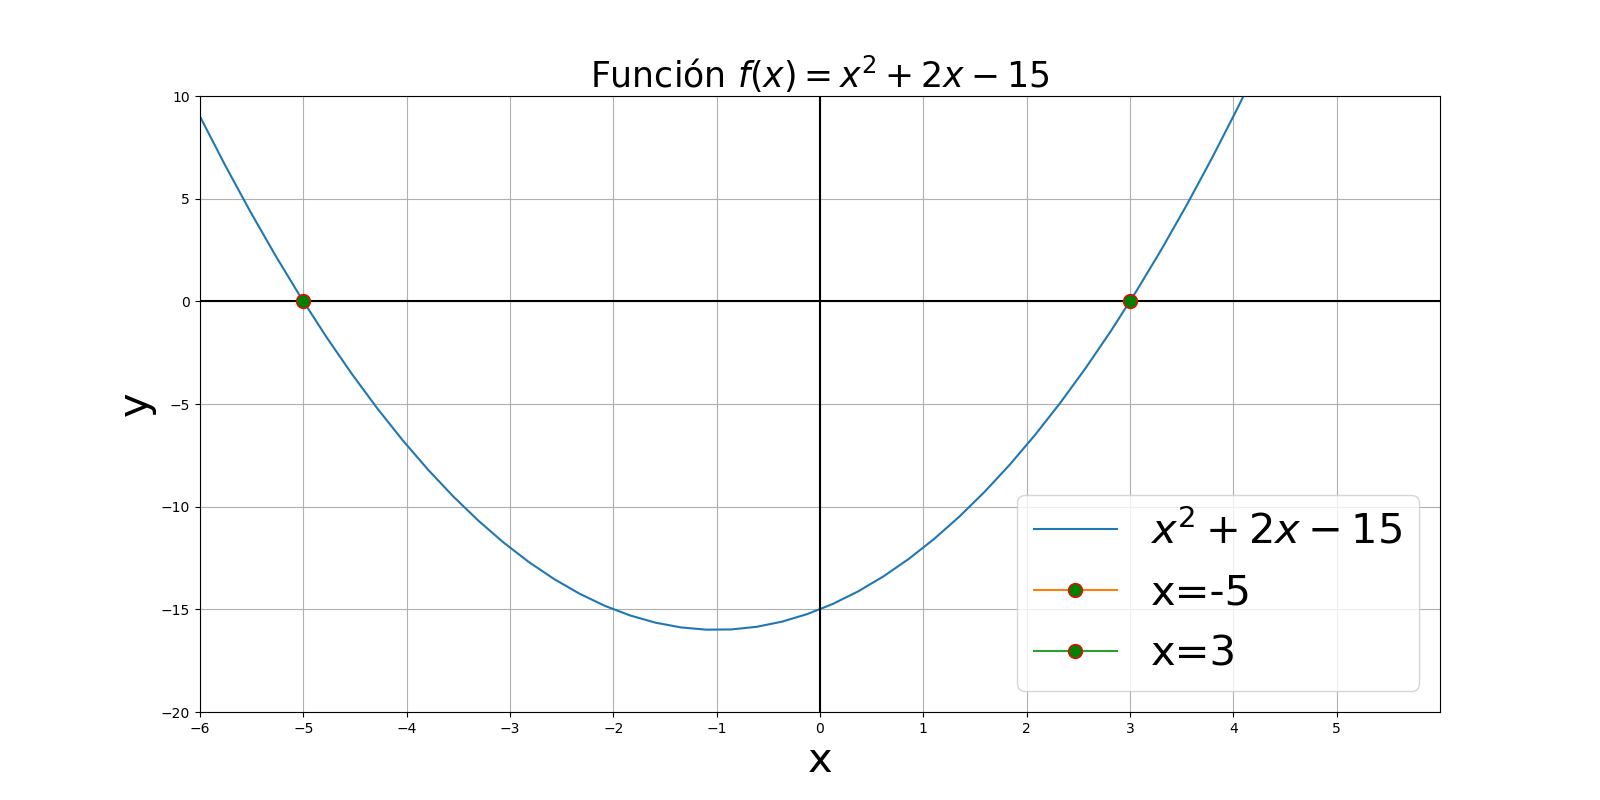
\includegraphics[scale=0.30]{cua441.png}
\caption[Gráfica de función cuadrática del ejemplo (\ref{ejem441}).]{Gráfica de función cuadrática del ejemplo (\ref{ejem441}). La expresión cuadrática tiene dos puntos de intersección con el eje $x$, que son justamente en donde cambia de signo los intervalos. }
\end{figure}
\end{center}
La desigualdad solicita que sea mayor que cero, por lo que los intervalos solución son $]-\infty,-5]\cup [3,+\infty[$. Los infinitos siempre son intervalos abiertos, en los otros casos lo determina el símbolo de la desigualdad (en este caso es un intervalo cerrado por el símbolo de la igualad).
\end{myexample}

Para las expresiones fraccionales con polinomios el procedimiento es análogo, pero hay que considerar que el denominador debe ser $\neq 0$.\\

\begin{myexample}
\label{ejemplo442}
Resolver la siguiente desigualdad fraccional:\\
\begin{eqnarray}
\dfrac{x+1}{x+3}+1&\leq &0 \\
\dfrac{x+1+x+3}{x+3} &\leq &0 \\
\dfrac{2x+4}{x+3}& \leq & 0 
\end{eqnarray} 
Los ceros son $x\neq-3$ y $x=-2$. Ahora se hace la tabla de signos con los ceros encontrados.\\
\begin{center}
\begin{table}[h!]
\centering
\begin{tabular}{|c|c|c|}
\hline
$-\infty$ a $-3$&$-3$ a $-2$& $-2$ a $+\infty$ \\
\hline
$x=-10$&$x=-2,5=-5/2$&$0$ \\
$\dfrac{(-)}{(-)}=+$&$\dfrac{(-)}{(+)}=-$&$\dfrac{(+)}{(+)}=+$ \\
\hline 
\end{tabular}
\caption[Tabla de signos de una inecuación fraccional.]{Tabla de signos de una inecuación fraccional.}
\end{table}
\end{center}
El intervalo que cumple con la condición de la desigualdad es $]-3,-2]$. Notar que el intervalo debe ser abierto en $-3$ y cerrado $-2$, o si no la desigualdad queda indefinida.
\end{myexample}

\begin{center}
\begin{figure}[h!]
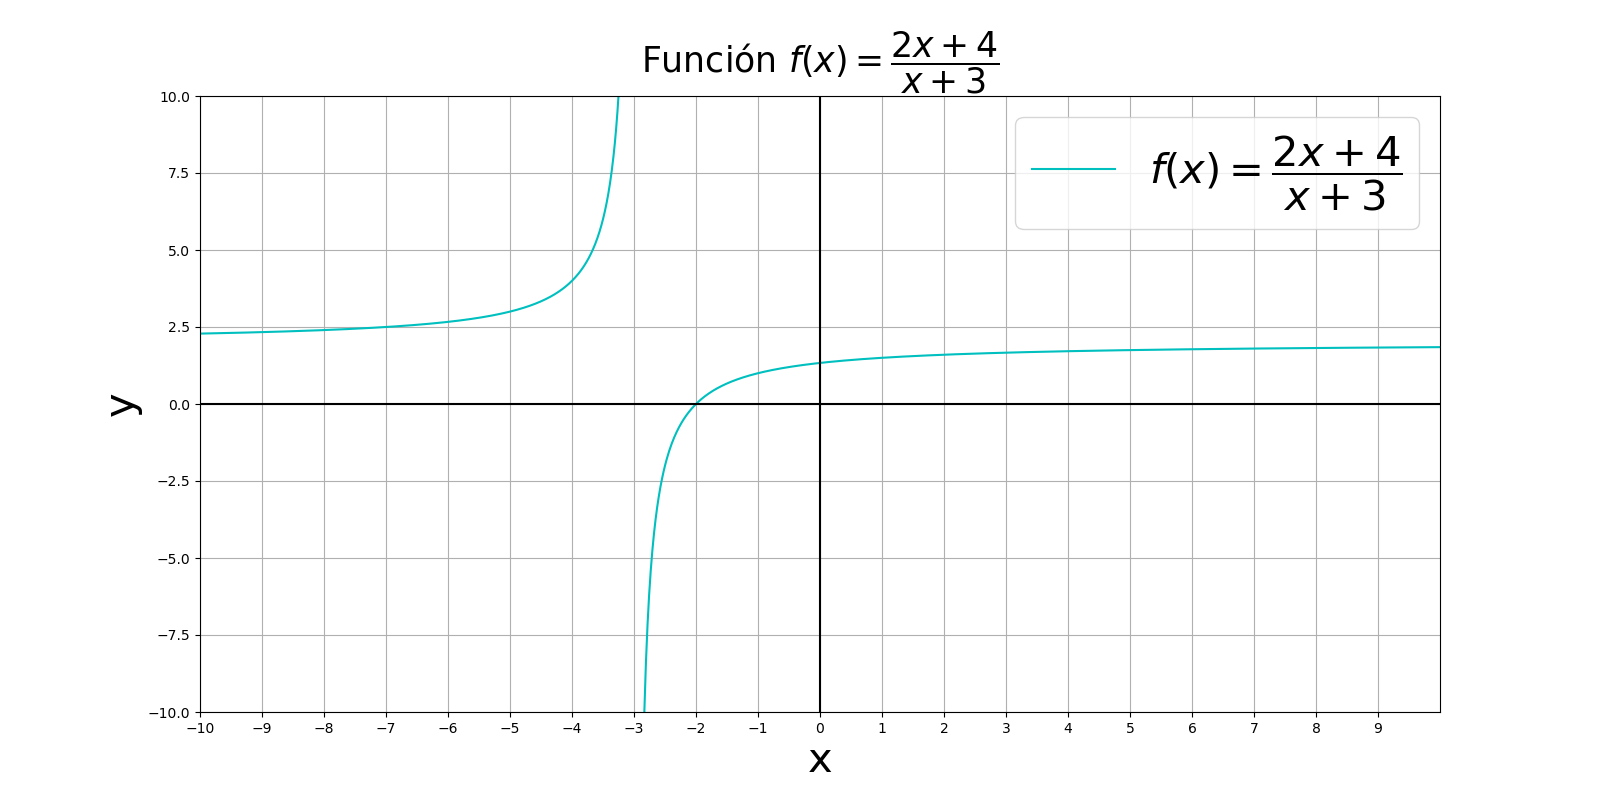
\includegraphics[scale=0.30]{inefracc0.png}\caption[Gráfico del ejemplo (\ref{ejemplo442}).]{Gráfico del ejemplo (\ref{ejemplo442}). Se Muestra (nuevamente) el intervalo en que la función cumple con la condición de la desigualdad (menor que cero, $\leq 0$).}
\end{figure}
\end{center}
\newpage
\subsection{Desigualdades polinomiales con valor absoluto}
Para finalizar el análisis de las desigualdades racionales, veremos el caso cuando tienen un valor absoluto. El procedimiento es el mismo solo que ahora se debe tener en consideración que habrán dos tablas con su (o sus) respectivo(s) conjunto(s) solución (o soluciones), que se deben unir. Luego, los conjuntos de las tablas se deberán intersectar o unir según el caso de valor absoluto. Ver el segundo ejercicio del ejemplo (\ref{ejemplodosd}).


\begin{myexample}
Resolver las siguientes expresiones polinomiales de fracciones con valor absoluto.\\

\noindent\textit{i)}
\begin{eqnarray*}
\left|\dfrac{1}{x}+3 \right| &\leq &3 \\
-3\leq &\dfrac{1}{x}+3& \leq 3 \\
-3\leq \dfrac{1}{x}+3 &\wedge &\dfrac{1}{x}+1 \leq 1 \\
0\leq \dfrac{1}{x}+6 &\wedge &\dfrac{1}{x} \leq 0\\
\underbrace{0\leq \dfrac{1+6x}{x}}_\text{$x\neq 0$,  $x=-1/6$} &\wedge &\underbrace{\dfrac{1}{x}\leq 0}_\text{$x\neq 0$}\\
\end{eqnarray*}

\begin{minipage}{0.5\textwidth}
\begin{tabular}{|c|c|c|}
\hline
  $-\infty$ a $-1/6$ & $-1/6$ a $0$ & $0$ a $+\infty$ \\
\hline
 $x=-10$ & $x-1/12$ & $x=10$  \\
  $\dfrac{(-)}{(-)}=+$&$\dfrac{(+)}{(-)}=-$&$\dfrac{(+)}{(+)}=+$  \\
\hline
\end{tabular}
\end{minipage}
\begin{minipage}{0.5\textwidth}
\begin{tabular}{|c|c|}
\hline
 $-\infty$ a $0$ & $0$ a $\infty$    \\
\hline
 $x=-1$&$x=1$   \\
  $\dfrac{(1)}{(-)}=-$& $\dfrac{(1)}{(+)}=+$  \\
  \hline
\end{tabular}
\end{minipage}

Ahora se debe hacer la intersección de ambas tablas, resultando como conjunto solución $\left( ]-\infty,-1/6]\cup ]0,+\infty[\right) \cap ]-\infty,0[=]-\infty,-1/6]$.\\
\begin{center}
\begin{figure}[h!]
\centering
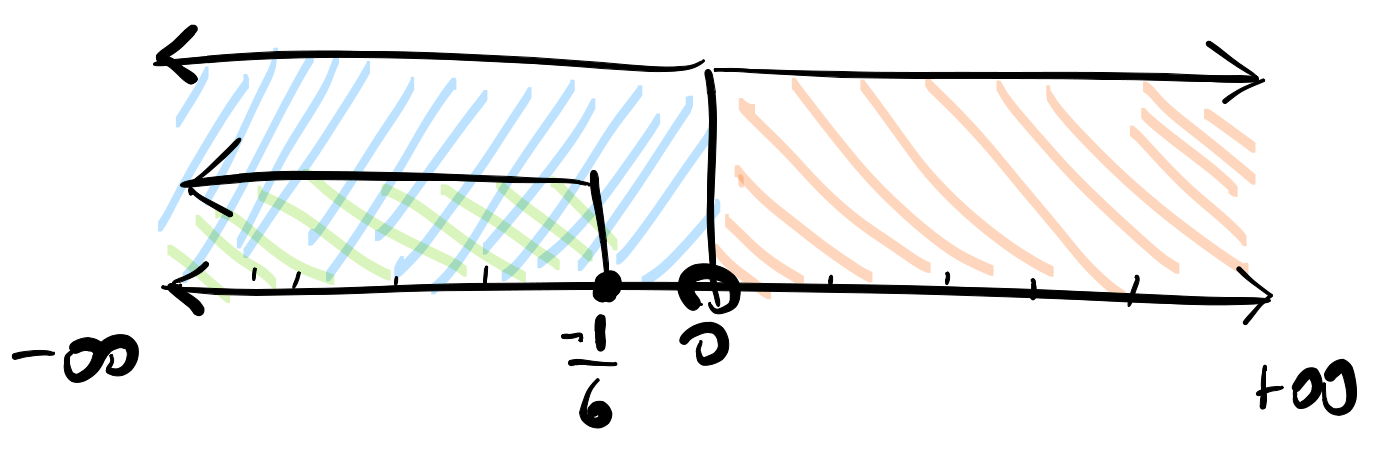
\includegraphics[scale=0.25]{Desabsfracc0.png}
\caption[Gráfica de los intervalos en la recta de los números reales.]{Gráfica de los intervalos en la recta de los números reales. Siempre se dibujan todos los  intervalos que cumplen la condición de la desigualdad (mayor o menor que 0).}
\end{figure}
\end{center}

\noindent\textit{ii)}\\
\begin{eqnarray*}
\left|\dfrac{3x-1}{x}\right| &\geq &4  \\
\dfrac{3x-1}{x}\geq 4 &\vee & \dfrac{3x-1}{x}\leq -4\\
\dfrac{3x-1}{x}-4\geq 0 &\vee & \dfrac{3x-1}{x}+4\leq 0\\
\dfrac{3x-1-4x}{x}\geq 0 &\vee & \dfrac{3x-1+4x}{x}\leq 0\\
\underbrace{\dfrac{-1-x}{x}\geq 0}_{x\neq 0, x=-1} &\vee & \underbrace{\dfrac{7x-1}{x}\leq 0}_{x\neq 0, x=1/7}
\end{eqnarray*}
\end{myexample}

\begin{minipage}{0.5\textwidth}
\begin{tabular}{|c|c|c|}
\hline
  $-\infty$ a $-1$ & $-1$ a $0$ & $0$ a $+\infty$ \\
\hline
 $x=-10$ & $x=-1/2$ & $x=10$  \\
  $\dfrac{(+)}{(-)}=-$&$\dfrac{(-)}{(-)}=+$&$\dfrac{(-)}{(+)}=-$\\
\hline
\end{tabular}
\end{minipage}
\begin{minipage}{0.5\textwidth}
\begin{tabular}{|c|c|c|}
\hline
 $-\infty$ a $0$ & $0$ a $1/7$& $1/7$ a $+\infty$    \\
\hline
 $x=-1$&$x=1/14$&$x=10$   \\
  $\dfrac{(-)}{(-)}=+$& $\dfrac{(-)}{(+)}=-$& $\dfrac{(+)}{(+)}=+$ \\
  \hline
\end{tabular}
\end{minipage}

En este caso debemos unir todos los resultados. De ambas tablas solo sirve un intervalo de cada una, entonces el conjunto solución es $[-1,0[\cup ]0,1/7]=[-1,1/7]-\{0\}$.

\begin{center}
\begin{figure}[h!]
\centering
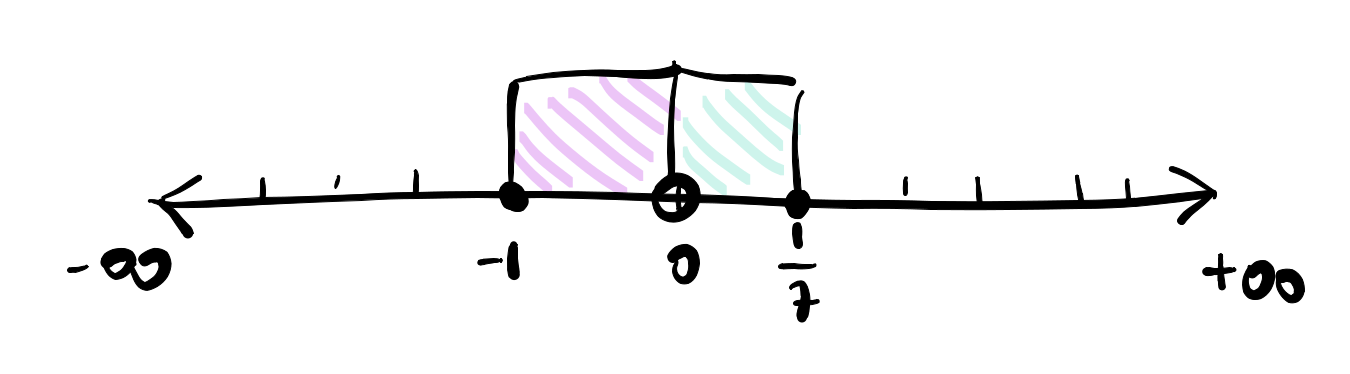
\includegraphics[scale=0.25]{Desabsfracc1.png}
\caption[Gráfica de los intervalos en la recta de los números reales.]{Gráfica de los intervalos en la recta de los números reales. Procedimiento similar al ejemplo anterior, solo que en este caso se debe unir los intervalos en vez de intersectarlos.}
\end{figure}
\end{center}